\begin{figure*}[t]
  \centering
  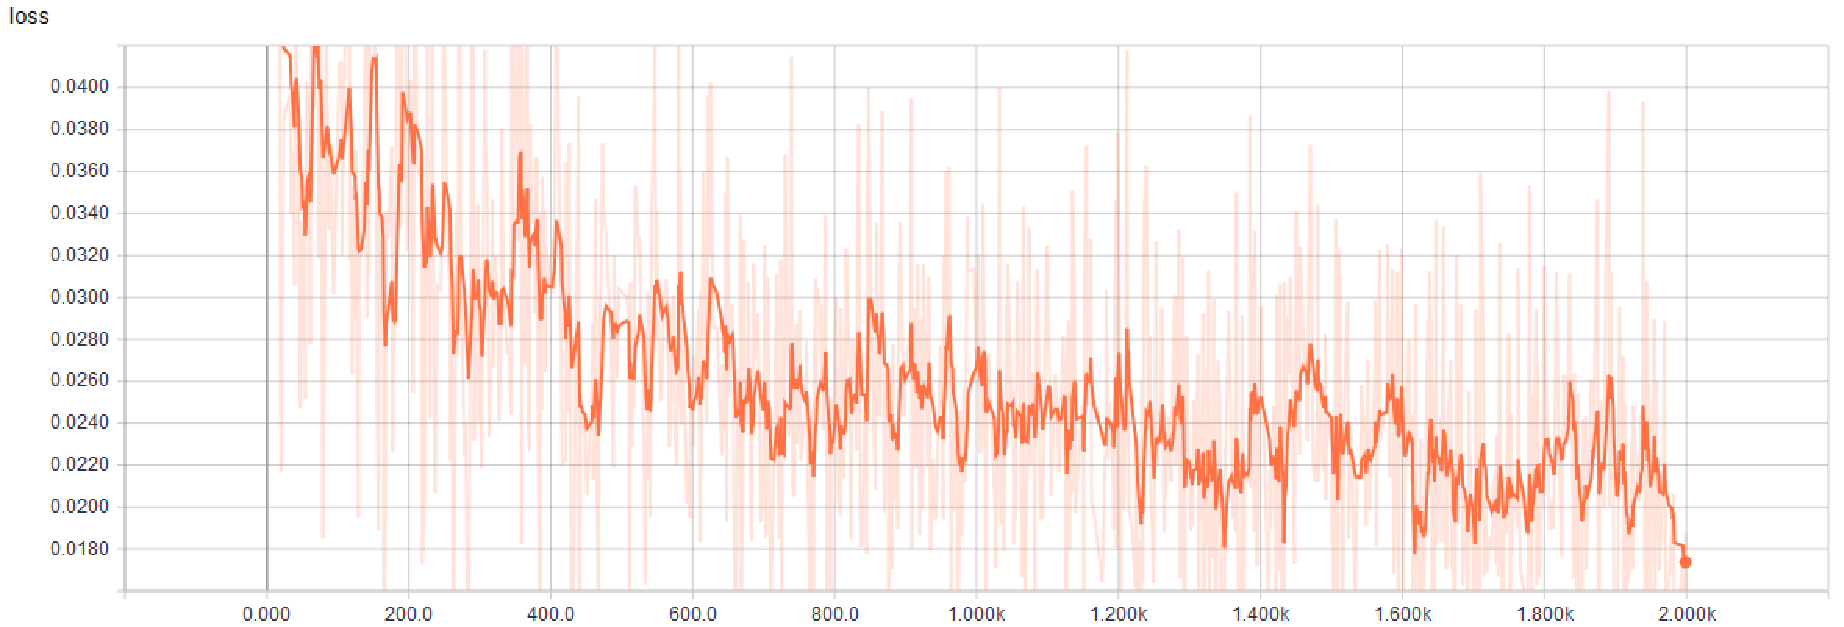
\includegraphics[width=.9\textwidth]{figs/TrainingLoss}
  \caption{Change in loss value throughout training.}
  \label{fig:modelloss}
\end{figure*}

\subsection{DNN Training and Testing}
We have trained and tested the deep neural network with several
different track conditions, different combinations of input
data, and different hyper parameters. In the following paragraphs, we 
describe details on two of the training methods that performed 
reasonably well.

In the first method, we trained the neural network model across a set 
of 30 completed runs on the track seen in Figure~\ref{fig:track2} by a
human pilot. Half of the runs saw the car driving one way along the
track, while the remaining half were of the car driving in the
opposite direction on the track.
In total, we collected 2,556 frames for training and 2,609 
frames for validation.
The weights of the network are initialized using a Xavier
initializer~\cite{Glorot2010}, which is known to provide better
initial values than the random weight assignment method.
In each training step, we use a batch
size of 100 frames, which are randomly selected among all the
collected training images, to optimize the network.
We repeat this across 2,000 training steps.
%% When a model was trained
%% with the  aformentioned data, the training loss was 0.0188 and the
%% validation  loss was 0.0132.
Figure~\ref{fig:modelloss} shows the change of the loss value over the
course of model training.

In the second method, we use the same data and parameters as  above 
except that now images are labeled as `curved' and `straight' and we pick an
equal number of images from each category at each training step to
update the model. In other words, we try to remove bias in selecting
images. We find that the car performed better in practice by applying
this approach as the car displayed a greater ability to stay in the
center of the track (on the white tape).
However, we find that there is a discrepency between the training
loss and the validation loss, indicating that the model may suffer
from an overfitting problem, despite its better real-world
performance.

%% as the former was 0.009, while the latter
%% was 0.0869

We plan to investigate ways to achieve better prediction accuracy
in training the network. We also plan to evaluate different RC
car platforms that have different steering mechanisms to see their
impact to the control performance.

\subsection{System-level Factors Affecting Real-Time Performance}
In using the Raspberry Pi 3 platform, there are a
few system-level factors, namely power supply and temperature, that
need to be considered to achieve consistent performance. 

In all our experiments on the Raspberry Pi 3, the CPU  is configured
at the maximum clock speed of 1.2 GHz. However, without care, it is
possible for the CPU to operate at a lower frequency involuntarily. 
An important factor is CPU thermal throttling, which can affect CPU
clock speed if the CPU temperature is too high (Pi 3's firmware is
configured to throttle at 85 deg. C).
DNN inferencing is computationally intensive, thus the temperature of
the CPU could rise quickly. This can be especially problematic in
situations where multiple DNN models run simultaneously on the
Pi 3. If the temperature reaches the threshold, the Pi 3's thermal
throttling kicks in and decreases the clock speed down to 600MHz---
half of the maximum 1.2GHz---so that the CPU's temperature stays at a
safe level.
We found that without proper cooling solutions (heatsink or fan), 
prolonged use of the system would result in CPU frequency decrease
that may affect evaluation.

Another factor to consider is power supply. From our experiences, the
Pi 3 frequency throttling also kicks in when the power source can not
provide the required minimum of 2A current.
In experiments conducted with a power supply that only provided 1 Amp,
the Pi was unable to sustain a 1.2 GHz clock speed, and instead,
fluctuated between operating at 600 MHz and 1.2 GHz. As a result, it
is necessary, or at least highly recommended, that the power supply
used for the Raspberry Pi 3 be capable of outputting 2 Amps, otherwise
optimal performance isn't guaranteed.

Our initial experiment results suffered from these issues, after which
we always carefully monitored the current operating frequencies of the
CPU cores during the experiments to ensure the correctness and
repeatability of the results.
